% Auto-generated from committed gate JSONs by generate_figures.py. Do not edit by hand.

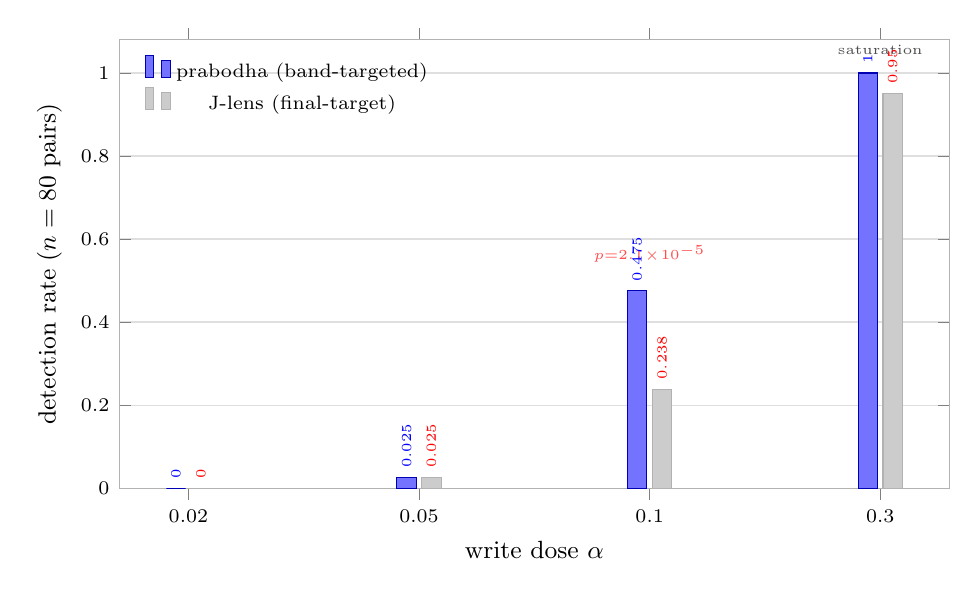
\begin{tikzpicture}
\begin{axis}[
  ybar, /pgf/bar width=7pt,
  width=\columnwidth, height=0.6\columnwidth,
  symbolic x coords={0.02,0.05,0.1,0.3},
  xtick=data, xlabel={write dose $\alpha$},
  ymin=0, ymax=1.08, ylabel={detection rate ($n=80$ pairs)},
  label style={font=\small}, tick label style={font=\scriptsize},
  legend style={font=\scriptsize, at={(0.02,0.98)}, anchor=north west, draw=none, fill=none},
  ymajorgrids, grid style={gray!25}, axis line style={gray!60},
  nodes near coords, nodes near coords style={font=\tiny, /pgf/number format/fixed, /pgf/number format/precision=3},
  every node near coord/.append style={rotate=90, anchor=west},
]
\addplot+[fill=blue!55, draw=blue!70!black] coordinates {(0.02,0.0) (0.05,0.025) (0.1,0.475) (0.3,1.0)};
\addplot+[fill=gray!40, draw=gray!60] coordinates {(0.02,0.0) (0.05,0.025) (0.1,0.2375) (0.3,0.95)};
\addlegendentry{prabodha (band-targeted)}
\addlegendentry{J-lens (final-target)}
\node[font=\tiny, red!70, anchor=south] at (axis cs:0.1,0.52) {$p{=}2.1\!\times\!10^{-5}$};
\node[font=\tiny, gray!60!black, anchor=south] at (axis cs:0.3,1.02) {saturation};
\end{axis}
\end{tikzpicture}
